\documentclass{article}

% Packages required by doxygen
\usepackage{calc}
\usepackage{doxygen}
\usepackage{graphicx}
\usepackage[utf8]{inputenc}
\usepackage{makeidx}
\usepackage{multicol}
\usepackage{multirow}
\usepackage{textcomp}
\usepackage[table]{xcolor}

% NLS support packages
\usepackage{polski}
\usepackage[T1]{fontenc}

% Font selection
\usepackage[T1]{fontenc}
\usepackage{mathptmx}
\usepackage[scaled=.90]{helvet}
\usepackage{courier}
\usepackage{amssymb}
\usepackage{sectsty}
\renewcommand{\familydefault}{\sfdefault}
\allsectionsfont{%
  \fontseries{bc}\selectfont%
  \color{darkgray}%
}
\renewcommand{\DoxyLabelFont}{%
  \fontseries{bc}\selectfont%
  \color{darkgray}%
}

% Page & text layout
\usepackage{geometry}
\geometry{%
  a4paper,%
  top=2.5cm,%
  bottom=2.5cm,%
  left=2.5cm,%
  right=2.5cm%
}
\tolerance=750
\hfuzz=15pt
\hbadness=750
\setlength{\emergencystretch}{15pt}
\setlength{\parindent}{0cm}
\setlength{\parskip}{0.2cm}
\makeatletter
\renewcommand{\paragraph}{%
  \@startsection{paragraph}{4}{0ex}{-1.0ex}{1.0ex}{%
    \normalfont\normalsize\bfseries\SS@parafont%
  }%
}
\renewcommand{\subparagraph}{%
  \@startsection{subparagraph}{5}{0ex}{-1.0ex}{1.0ex}{%
    \normalfont\normalsize\bfseries\SS@subparafont%
  }%
}
\makeatother

% Headers & footers
\usepackage{fancyhdr}
\pagestyle{fancyplain}
\fancyhead[LE]{\fancyplain{}{\bfseries\thepage}}
\fancyhead[CE]{\fancyplain{}{}}
\fancyhead[RE]{\fancyplain{}{\bfseries\leftmark}}
\fancyhead[LO]{\fancyplain{}{\bfseries\rightmark}}
\fancyhead[CO]{\fancyplain{}{}}
\fancyhead[RO]{\fancyplain{}{\bfseries\thepage}}
\fancyfoot[LE]{\fancyplain{}{}}
\fancyfoot[CE]{\fancyplain{}{}}
\fancyfoot[RE]{\fancyplain{}{\bfseries\scriptsize Wygenerowano N, 15 mar 2015 20\-:19\-:16 dla Lab01 -\/ mnożenie przez 2 programem Doxygen }}
\fancyfoot[LO]{\fancyplain{}{\bfseries\scriptsize Wygenerowano N, 15 mar 2015 20\-:19\-:16 dla Lab01 -\/ mnożenie przez 2 programem Doxygen }}
\fancyfoot[CO]{\fancyplain{}{}}
\fancyfoot[RO]{\fancyplain{}{}}
\renewcommand{\footrulewidth}{0.4pt}
\renewcommand{\chaptermark}[1]{%
  \markboth{#1}{}%
}
\renewcommand{\sectionmark}[1]{%
  \markright{\thesection\ #1}%
}

% Indices & bibliography
\usepackage{natbib}
\usepackage[titles]{tocloft}
\setcounter{tocdepth}{3}
\setcounter{secnumdepth}{5}
\makeindex

% Hyperlinks (required, but should be loaded last)
\usepackage{ifpdf}
\ifpdf
  \usepackage[pdftex,pagebackref=true]{hyperref}
\else
  \usepackage[ps2pdf,pagebackref=true]{hyperref}
\fi
\hypersetup{%
  colorlinks=true,%
  linkcolor=blue,%
  citecolor=blue,%
  unicode%
}

% Custom commands
\newcommand{\clearemptydoublepage}{%
  \newpage{\pagestyle{empty}\cleardoublepage}%
}


%===== C O N T E N T S =====

\begin{document}

% Titlepage & ToC
\hypersetup{pageanchor=false}
\pagenumbering{roman}
\begin{titlepage}
\vspace*{7cm}
\begin{center}%
{\Large Lab01 -\/ mnożenie przez 2 }\\
\vspace*{1cm}
{\large Mateusz Krawczuk, nr indeksu 209147}\\
\vspace{0.5cm}
{\large Wygenerowano przez Doxygen 1.8.6}\\
\vspace*{0.5cm}
{\small N, 15 mar 2015 20:19:16}\\
\end{center}
\end{titlepage}
%\clearemptydoublepage
%\tableofcontents
%\clearemptydoublepage
\pagenumbering{arabic}
%\hypersetup{pageanchor=true}

%--- Begin generated contents ---
\part{Streszczenie}
Niniejszy dokument zawiera wyniki pomiaru czasu, którego potrzebował mój komputer na zapełnienie zaimplementowanych przeze mnie struktur danych opartych na typach tablicowych: stos, kolejka oraz lista zestawami danych o długościach od 1 do 1e7 elementów. Zawiera także dokumentację kodu, który pojawił się w projekcie od poprzedniego sprawozdania.

\part{Sprawozdanie}
Obliczenia wykonano na 64-bitowym procesorze AMD Athlon X2. Wszystkie implementacje zostały badane pod kątem najgorszego scenariusza. Wykresy przedstawiają porównania zależnośći czasu wykonywania operacji od długości ciągu danych dla różnych implementacji poszczególnych struktur. Porównywane implementacje to: \newline
- kontenery z biblioteki standardowej, \newline
- implementacja z użyciem list jednokierunkowych, \newline
- z użyciem tablic, gdzie pojemność tablicy jest zwiększana o jeden element,\newline
- z użyciem tablic, gdzie pojemność tablicy zwiększana jest dwukrotnie.
\vspace{0.5cm}
\newpage
\centerline{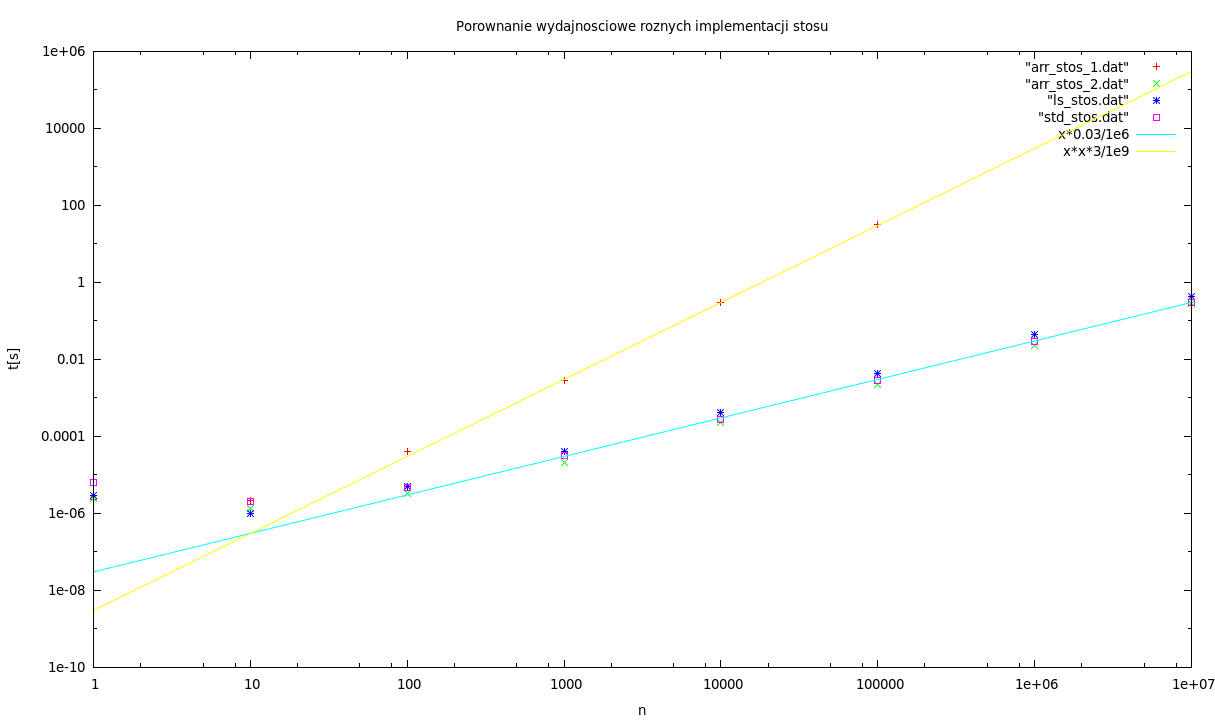
\includegraphics[width=\textwidth,height=\textheight, keepaspectratio]{stos.png}}
Wykres 1. Porównanie różnych implementacji stosu.
\newline
% ### KOMENTARZ DO 1. WYKRESU
Zależność czasu wykonywania operacji od ilości danych wrzucanych na szczyt stosu dla wszystkich implementacji z wyjątkiem tablicowej-zwiększanej-o-1 dobrze aproksymuje linia prosta po czym można przypuszczać, że złożoność tej operacji jest \begin{math}O(n)\end{math}. Dla stosu z biblioteki standardowej i zaimplementowanego za pomocą listy jest to trafny wniosek, gdyż ich złożoność jest faktycznie liniowa. Inaczej jest w przypadku stosu tablicowego-powiększanego-dwukrotnie, bowiem w trakcie powiększania go co jakiś czas następuje przepisanie całej jego zawartośći do innego miejsca w pamięci, co oczywiście jest operacją liniową. Jednak w związku z tym, że wraz ze zwiększaniem się ilości danych na stosie częstotliwość wystąpienia operacji przenoszenia maleje, wzrasta wydajność czasowa kosztem wydajności pamięciowej. Jak widać na wykresie, prosta bardzo dobrze aproksymuje stopień złożoności dla tej implementacji.

W przypadku stosu tablicowego-powiększanego-o-1 za każdym razem, gdy wyczerpiemy zapas pojemności kontenera, następuje realokacja całej jego zawartości do nowego miejsca z zapasem mogącym zmieścić jeden element - ten zapas wyczerpuje się w momencie, w którym wrzucimy na stos kolejny element. W konsekwencji wrzucenie na stos \begin{math}n\end{math} danych kosztuje nas \begin{math}n\end{math}-krotne \begin{math}n\end{math} przepisań całego stosu, co razem daje \begin{math}n^{2}\end{math} operacji, zatem złożoność obliczeniowa tego przedsięwzięcia wynosi \begin{math}O(n^{2})\end{math}.Gdyby wykres był w skali liniowej, linia aproksymująca współrzędne uzyskane z badań nad tą implementacją byłaby ramieniem paraboli.
\newpage
\centerline{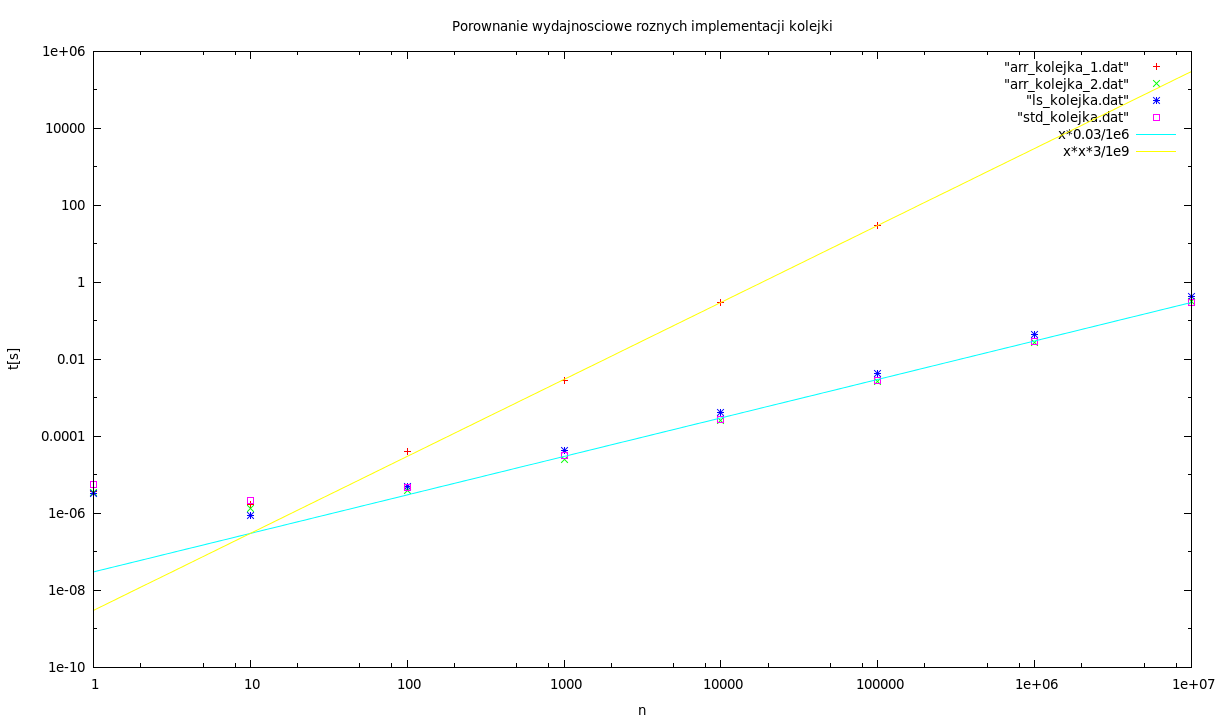
\includegraphics[width=\textwidth,height=\textheight, keepaspectratio]{kolejka.png}}
Wykres 2. Porównanie różnych implementacji kolejki.
\newline
% ### KOMENTARZ DO 2. WYKRESU

Sytuacja jest identyczna jak w przypadku stosu - ze względu na sposób implementacji wyniki są prawie identyczne. Różnice w tych strukturach byłyby widoczne, gdyby badano zdejmowanie z nich elementów.
\newpage
\centerline{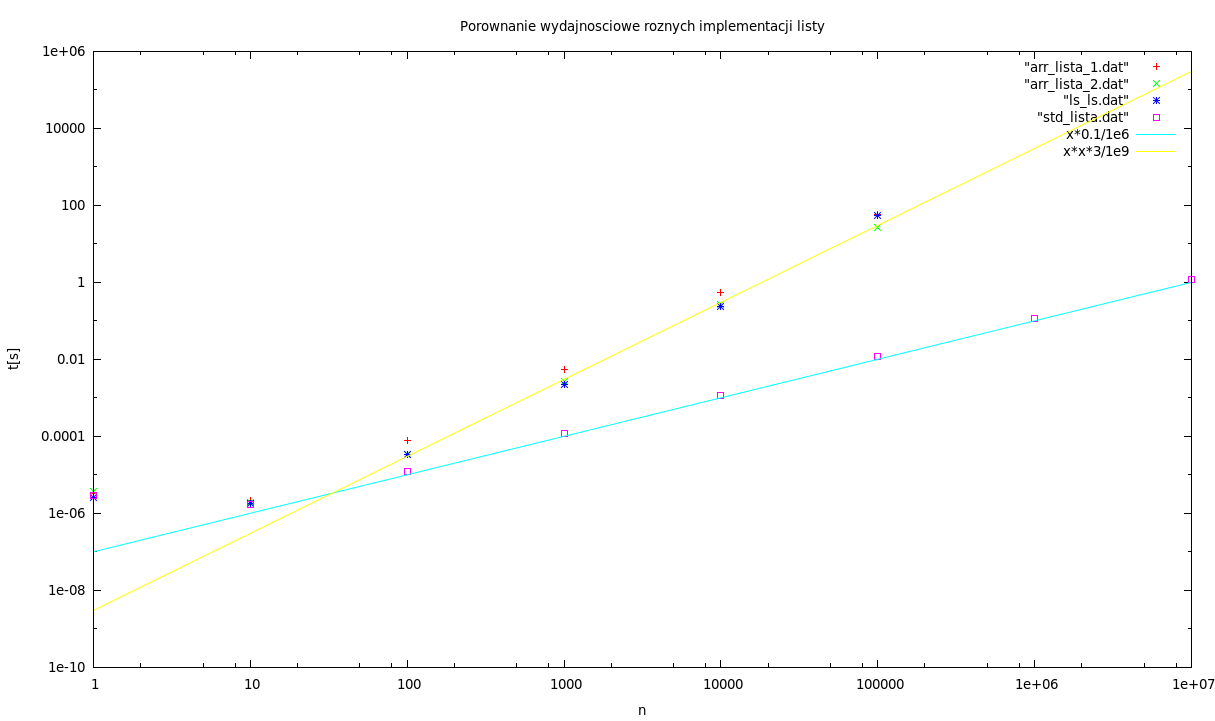
\includegraphics[width=\textwidth,height=\textheight, keepaspectratio]{lista.png}}
Wykres 3. Porównanie różnych implmentacji listy.
\newline
% ### KOMENTARZ DO 3. WYKRESU
Jedyną implementacją, w której umieszczanie elementów ma złożoność liniową jest lista z biblioteki standardowej. Jest to spodowane tym, że std::list wykorszytane do porównania jest listą dwukierunkową i nie jest wymagane każdorazowe przesuwanie jej zawartości podczas dodawania do niej elementu.

Złożoność obliczeniowa wszystkich moich implementacji jest \begin{math}O(n^{2})\end{math}, ponieważ napisana przez mnie lista jednokierunkowa została zaprojektowana w taki sposób, że dodawanie na jej początek nowego elementu (co jest najgorszym scenariuszem pod względem złożoności) wymaga operacji na każdym elemencie istniejącym w liście - jest to przesuwanie wskaźnika pomocniczego z końca na sam początek listy lub podnoszenie każdego elementu o jedno miejsce bliżej końca. Mamy więc dla \begin{math}n\end{math}-elemenotwego zbioru danych \begin{math}n\end{math}-krotne\begin{math} n\end{math} przesunięć wektora służące wpięciu nowego elementu listy na jej początek lub, w przypadku implementacji tablicowej, \begin{math}n\end{math}-krotne \begin{math}n\end{math} podniesień elementów bliżej końca by zrobić miejsce na nowy element w indeksie zerowym. 
\newpage

\part{Dokumentacja kodu}
\hypertarget{benchmark_8h}{\section{benchmark.\-h File Reference}
\label{benchmark_8h}\index{benchmark.\-h@{benchmark.\-h}}
}


Deklaracje funkcji związanych z analizą prędkości operacji.  


{\ttfamily \#include \char`\"{}operacja.\-h\char`\"{}}\\*
{\ttfamily \#include \char`\"{}ustawienia.\-h\char`\"{}}\\*
{\ttfamily \#include \char`\"{}kontener.\-h\char`\"{}}\\*
{\ttfamily \#include \char`\"{}stos.\-h\char`\"{}}\\*
{\ttfamily \#include \char`\"{}kolejka.\-h\char`\"{}}\\*
{\ttfamily \#include \char`\"{}stos\-\_\-arr.\-h\char`\"{}}\\*
{\ttfamily \#include $<$fstream$>$}\\*
{\ttfamily \#include $<$iostream$>$}\\*
{\ttfamily \#include $<$vector$>$}\\*
{\ttfamily \#include $<$cstdlib$>$}\\*
{\ttfamily \#include $<$cmath$>$}\\*
\subsection*{Functions}
\begin{DoxyCompactItemize}
\item 
void \hyperlink{benchmark_8h_aa64f5c659f0dd5f25435b15c1e1fa7f5}{Benchmark} ()
\begin{DoxyCompactList}\small\item\em Główna funkcja programu. \end{DoxyCompactList}\item 
int \hyperlink{benchmark_8h_a43bc241c88791024a92dc76ff18d0d48}{licz\-\_\-dekady} (int dlugosc\-\_\-ciagu)
\begin{DoxyCompactList}\small\item\em Funkcja pomocnicza do określania ilości dekad. \end{DoxyCompactList}\end{DoxyCompactItemize}


\subsection{Detailed Description}
Plik zawiera deklaracje funkcji \hyperlink{benchmark_8h_aa64f5c659f0dd5f25435b15c1e1fa7f5}{Benchmark()} oraz \hyperlink{benchmark_8h_a43bc241c88791024a92dc76ff18d0d48}{licz\-\_\-dekady()}. Funkcja \hyperlink{benchmark_8h_aa64f5c659f0dd5f25435b15c1e1fa7f5}{Benchmark()} jest główną funkcją programu benchmarkującego, natomiast funkcja \hyperlink{benchmark_8h_a43bc241c88791024a92dc76ff18d0d48}{licz\-\_\-dekady()} jest funkcją pomocniczą wywoływaną w funkcji \hyperlink{benchmark_8h_aa64f5c659f0dd5f25435b15c1e1fa7f5}{Benchmark()}. 

Definition in file \hyperlink{benchmark_8h_source}{benchmark.\-h}.



\subsection{Function Documentation}
\hypertarget{benchmark_8h_aa64f5c659f0dd5f25435b15c1e1fa7f5}{\index{benchmark.\-h@{benchmark.\-h}!Benchmark@{Benchmark}}
\index{Benchmark@{Benchmark}!benchmark.h@{benchmark.\-h}}
\subsubsection[{Benchmark}]{\setlength{\rightskip}{0pt plus 5cm}void Benchmark (
\begin{DoxyParamCaption}
{}
\end{DoxyParamCaption}
)}}\label{benchmark_8h_aa64f5c659f0dd5f25435b15c1e1fa7f5}
Funkcja wywoływana w funkcji \hyperlink{main_8cpp_ae66f6b31b5ad750f1fe042a706a4e3d4}{main()}. Nie przyjmuje argumentów ani nie zwraca wartości. Funkcja otwiera plik, który powinien zawierać ciąg danych, na których przeprowadzona zostanie operacja. Otwiera także plik, do którego zapisane mają zostać wyniki czasowe operacji. Nazwy plików określone są w nagłówku \char`\"{}ustawienia.\-h\char`\"{}. Z pliku wejściowego wczytuje do obiektu klasy std\-::vector ciąg danych. Do zmiennej typu clock\-\_\-t zostaje zapisany czas procesora od rozpoczęcia procesu. Do funkcji \hyperlink{operacja_8h_a7de44f86b01513b6593ff27e0f62645e}{operacja()} zostaje przekazana referencja do obiektu zawierającego ciąg danych. Po wyjściu z funkcji \hyperlink{operacja_8h_a7de44f86b01513b6593ff27e0f62645e}{operacja()} do zmiennej typu clock\-\_\-t() zostaje tym razem zapisana różnica czasów procesora pomiędzy rozpoczęciem procesu a wartością typu clock\-\_\-t zwróconą przez funkcję \hyperlink{operacja_8h_a7de44f86b01513b6593ff27e0f62645e}{operacja()}. Czas ten przeliczany jest na sekundy i zapisany do pliku wyjściowego. W \char`\"{}ustawienia.\-h\char`\"{} określona jest ilość powtórzeń pomiaru. Pomiary zaczynają się od operacji na jednej wartości i kończą na ciąu danych o długości największej potęgi dziesiątki. Pomiary powtarzane są co dekadę. Informację o największej potędze dziesiątki dostarcza funkcja \hyperlink{benchmark_8h_a43bc241c88791024a92dc76ff18d0d48}{licz\-\_\-dekady()}. 

Definition at line 4 of file benchmark.\-cpp.

\hypertarget{benchmark_8h_a43bc241c88791024a92dc76ff18d0d48}{\index{benchmark.\-h@{benchmark.\-h}!licz\-\_\-dekady@{licz\-\_\-dekady}}
\index{licz\-\_\-dekady@{licz\-\_\-dekady}!benchmark.h@{benchmark.\-h}}
\subsubsection[{licz\-\_\-dekady}]{\setlength{\rightskip}{0pt plus 5cm}int licz\-\_\-dekady (
\begin{DoxyParamCaption}
\item[{int}]{dlugosc\-\_\-ciagu}
\end{DoxyParamCaption}
)}}\label{benchmark_8h_a43bc241c88791024a92dc76ff18d0d48}
Przyjmuje jako argument liczbę całkowitą reprezentującą długość ciągu danych i zaokrągla ją w dół do najbliższej potęgi liczby 10.


\begin{DoxyParams}[1]{Parameters}
\mbox{\tt in}  & {\em dlugosc\-\_\-ciagu} & Długość ciągu danych. \\
\hline
\end{DoxyParams}
\begin{DoxyReturn}{Returns}
Zwraca zaokrąglenie w dół do najbliższej potęgi dziesiątki wartości dlugosc\-\_\-ciagu. 
\end{DoxyReturn}


Definition at line 59 of file benchmark.\-cpp.


\hypertarget{operacja_8h}{\section{/home/damian/prog/\-Obserwator/prj/inc/operacja.h File Reference}
\label{operacja_8h}\index{/home/damian/prog/\-Obserwator/prj/inc/operacja.\-h@{/home/damian/prog/\-Obserwator/prj/inc/operacja.\-h}}
}
{\ttfamily \#include \char`\"{}Lista\-Ar.\-h\char`\"{}}\\*
\subsection*{Functions}
\begin{DoxyCompactItemize}
\item 
\hyperlink{class_ltab}{Ltab} \hyperlink{operacja_8h_a55fd4ff5b64240f5b5e352bf951d0eaf}{operacja} (\hyperlink{class_ltab}{Ltab} A, int l, int p)
\end{DoxyCompactItemize}


\subsection{Function Documentation}
\hypertarget{operacja_8h_a55fd4ff5b64240f5b5e352bf951d0eaf}{\index{operacja.\-h@{operacja.\-h}!operacja@{operacja}}
\index{operacja@{operacja}!operacja.h@{operacja.\-h}}
\subsubsection[{operacja}]{\setlength{\rightskip}{0pt plus 5cm}{\bf Ltab} operacja (
\begin{DoxyParamCaption}
\item[{{\bf Ltab}}]{A, }
\item[{int}]{l, }
\item[{int}]{p}
\end{DoxyParamCaption}
)}}\label{operacja_8h_a55fd4ff5b64240f5b5e352bf951d0eaf}


Definition at line 10 of file operacja.\-cpp.


\section{/home/damian/mkrawczuk/209147/lab03\-\_\-opt/prj/inc/ustawienia.h File Reference}
\label{ustawienia_8h}\index{/home/damian/mkrawczuk/209147/lab03\-\_\-opt/prj/inc/ustawienia.\-h@{/home/damian/mkrawczuk/209147/lab03\-\_\-opt/prj/inc/ustawienia.\-h}}


Plik zawiera stałe preprocesora związane z generowaniem, obróbką i pomiarem właściwości danych.  


\subsection*{Macros}
\begin{DoxyCompactItemize}
\item 
\#define {\bf I\-L\-O\-S\-C}~1e2
\item 
\#define {\bf K\-R\-E\-S\-\_\-\-G\-O\-R\-N\-Y}~100
\item 
\#define {\bf K\-R\-E\-S\-\_\-\-D\-O\-L\-N\-Y}~0
\item 
\#define {\bf N\-A\-Z\-W\-A\-\_\-\-P\-L\-I\-K\-U\-\_\-\-W\-E}~\char`\"{}dane.\-dat\char`\"{}
\item 
\#define {\bf N\-A\-Z\-W\-A\-\_\-\-P\-L\-I\-K\-U\-\_\-\-W\-Y}~\char`\"{}arr\-\_\-lista\-\_\-1.\-dat\char`\"{}
\item 
\#define {\bf I\-L\-O\-S\-C\-\_\-\-P\-O\-W\-T\-O\-R\-Z\-E\-N}~10
\end{DoxyCompactItemize}


\subsection{Detailed Description}
Plik zawiera stałe preprocesora związane z generowaniem, obróbką i pomiarem właściwości danych. Makra zawarte w tym pliku służą do sterowania pracą programu generującego dane oraz programu, który te dane przetwarza. Służy też synchronizacji pomiędzy tymi dwoma programami poprzez ujednolicenie nazwy pliku zawierającego dane. 

Definition in file {\bf ustawienia.\-h}.



\subsection{Macro Definition Documentation}
\index{ustawienia.\-h@{ustawienia.\-h}!I\-L\-O\-S\-C@{I\-L\-O\-S\-C}}
\index{I\-L\-O\-S\-C@{I\-L\-O\-S\-C}!ustawienia.h@{ustawienia.\-h}}
\subsubsection[{I\-L\-O\-S\-C}]{\setlength{\rightskip}{0pt plus 5cm}\#define I\-L\-O\-S\-C~1e2}\label{ustawienia_8h_a400f3b16594461b02b7a73ad07b24c0e}
Określa dłuość ciągu danych stworzonych przez program generuj. 

Definition at line 14 of file ustawienia.\-h.

\index{ustawienia.\-h@{ustawienia.\-h}!I\-L\-O\-S\-C\-\_\-\-P\-O\-W\-T\-O\-R\-Z\-E\-N@{I\-L\-O\-S\-C\-\_\-\-P\-O\-W\-T\-O\-R\-Z\-E\-N}}
\index{I\-L\-O\-S\-C\-\_\-\-P\-O\-W\-T\-O\-R\-Z\-E\-N@{I\-L\-O\-S\-C\-\_\-\-P\-O\-W\-T\-O\-R\-Z\-E\-N}!ustawienia.h@{ustawienia.\-h}}
\subsubsection[{I\-L\-O\-S\-C\-\_\-\-P\-O\-W\-T\-O\-R\-Z\-E\-N}]{\setlength{\rightskip}{0pt plus 5cm}\#define I\-L\-O\-S\-C\-\_\-\-P\-O\-W\-T\-O\-R\-Z\-E\-N~10}\label{ustawienia_8h_a923942350ba378e49a53193355cb5ec0}
Tyle razy zostanie powtórzoy pomiar dla jednego zestawu danych. 

Definition at line 24 of file ustawienia.\-h.

\index{ustawienia.\-h@{ustawienia.\-h}!K\-R\-E\-S\-\_\-\-D\-O\-L\-N\-Y@{K\-R\-E\-S\-\_\-\-D\-O\-L\-N\-Y}}
\index{K\-R\-E\-S\-\_\-\-D\-O\-L\-N\-Y@{K\-R\-E\-S\-\_\-\-D\-O\-L\-N\-Y}!ustawienia.h@{ustawienia.\-h}}
\subsubsection[{K\-R\-E\-S\-\_\-\-D\-O\-L\-N\-Y}]{\setlength{\rightskip}{0pt plus 5cm}\#define K\-R\-E\-S\-\_\-\-D\-O\-L\-N\-Y~0}\label{ustawienia_8h_a6b2bdad24a7530210341c1c3a0197dd9}
Określa najmniejszą możliwą liczbę do wygenerowania. 

Definition at line 18 of file ustawienia.\-h.

\index{ustawienia.\-h@{ustawienia.\-h}!K\-R\-E\-S\-\_\-\-G\-O\-R\-N\-Y@{K\-R\-E\-S\-\_\-\-G\-O\-R\-N\-Y}}
\index{K\-R\-E\-S\-\_\-\-G\-O\-R\-N\-Y@{K\-R\-E\-S\-\_\-\-G\-O\-R\-N\-Y}!ustawienia.h@{ustawienia.\-h}}
\subsubsection[{K\-R\-E\-S\-\_\-\-G\-O\-R\-N\-Y}]{\setlength{\rightskip}{0pt plus 5cm}\#define K\-R\-E\-S\-\_\-\-G\-O\-R\-N\-Y~100}\label{ustawienia_8h_a2e9c0e30a722750fa4380b8150337c6f}
Określa największą możliwą liczbę do wygenerowania. 

Definition at line 16 of file ustawienia.\-h.

\index{ustawienia.\-h@{ustawienia.\-h}!N\-A\-Z\-W\-A\-\_\-\-P\-L\-I\-K\-U\-\_\-\-W\-E@{N\-A\-Z\-W\-A\-\_\-\-P\-L\-I\-K\-U\-\_\-\-W\-E}}
\index{N\-A\-Z\-W\-A\-\_\-\-P\-L\-I\-K\-U\-\_\-\-W\-E@{N\-A\-Z\-W\-A\-\_\-\-P\-L\-I\-K\-U\-\_\-\-W\-E}!ustawienia.h@{ustawienia.\-h}}
\subsubsection[{N\-A\-Z\-W\-A\-\_\-\-P\-L\-I\-K\-U\-\_\-\-W\-E}]{\setlength{\rightskip}{0pt plus 5cm}\#define N\-A\-Z\-W\-A\-\_\-\-P\-L\-I\-K\-U\-\_\-\-W\-E~\char`\"{}dane.\-dat\char`\"{}}\label{ustawienia_8h_a38a14ca65ed113a739420d7a6813c0e8}
Określa jak nazywa się plik wygenerowany przez program 'generuj', jednocześnie pliku o tej nazwie poszukuje program 'program' w katalogu, w którym został uruchomiony. 

Definition at line 20 of file ustawienia.\-h.

\index{ustawienia.\-h@{ustawienia.\-h}!N\-A\-Z\-W\-A\-\_\-\-P\-L\-I\-K\-U\-\_\-\-W\-Y@{N\-A\-Z\-W\-A\-\_\-\-P\-L\-I\-K\-U\-\_\-\-W\-Y}}
\index{N\-A\-Z\-W\-A\-\_\-\-P\-L\-I\-K\-U\-\_\-\-W\-Y@{N\-A\-Z\-W\-A\-\_\-\-P\-L\-I\-K\-U\-\_\-\-W\-Y}!ustawienia.h@{ustawienia.\-h}}
\subsubsection[{N\-A\-Z\-W\-A\-\_\-\-P\-L\-I\-K\-U\-\_\-\-W\-Y}]{\setlength{\rightskip}{0pt plus 5cm}\#define N\-A\-Z\-W\-A\-\_\-\-P\-L\-I\-K\-U\-\_\-\-W\-Y~\char`\"{}arr\-\_\-lista\-\_\-1.\-dat\char`\"{}}\label{ustawienia_8h_af22a754e002d9be8ee0b6d97eb9a9882}
Tak nazywać się będzie wygenerowany przez program 'program' plik z wynikami przeprowadzonych pomiarów. 

Definition at line 22 of file ustawienia.\-h.


%--- End generated contents ---

% Index
\newpage
\phantomsection
\addcontentsline{toc}{chapter}{Indeks}
\printindex

\end{document}
